\documentclass[10pt]{sigplanconf}

\usepackage{amsmath}
\usepackage{natbib}
\usepackage{graphicx}
\usepackage{url}
\usepackage{listings}
\usepackage{color} 
 
\pdfpagewidth=8.5in
\pdfpageheight=11in

\begin{document}
 
\conferenceinfo{PLASTIC'11,} {October 24, 2011, Portland, Oregon, USA.}
\CopyrightYear{2011}
\copyrightdata{978-1-4503-1171-7/11/10}

\title{Enterprise JavaScript with Jangaroo}
\subtitle{Using ActionScript 3 for JavaScript "Programming in the Large"}

\authorinfo{Andreas Gawecki \and Frank Wienberg}
           {CoreMedia}
           {\{andreas.gawecki,frank.wienberg\}@coremedia.com}

\maketitle

\begin{abstract}
By compiling ActionScript 3 to JavaScript, the Open Source project Jangaroo lets web developers utilize a superior language for building large scale web applications. Since JavaScript is used as the target language, no browser plug-in is needed to run Jangaroo applications. Jangaroo reuses and provides professional tools supporting the complete software development lifecycle. CoreMedia uses the Jangaroo tool chain extensively to aid the development of CoreMedia Studio, a large scale web application which provides the user interface for the CoreMedia Web Content Management System. This paper gives an overview of Jangaroo and offers insight into concepts and inner workings of the Jangaroo compiler and runtime support.
\end{abstract}

\category{D.2.3}{Software Engineering}{
Coding Tools and Techniques}
\category{D.2.11}{Software Engineering}{
Software Architectures }
\category{D.3.3}{Programming Languages}{
Language Constructs and Features -- Classes and objects, Frameworks, Inheritance, Modules, packages}
\category{D.3.4}{Programming Languages}{
Processors --- Code generation, Compilers, Debuggers, Parsing, Run-time environments}

\terms
Languages, Documentation, Standardization 

\keywords
JavaScript; ActionScript;
RIA; \\
Programming in the large; 
Browser; Opensource, Compilers; 
Flash

\section{Introduction}

Jangaroo (\texttt{www.jangaroo.net}) is a set of tools which bring enterprise language features to JavaScript programmers. This includes classes and inheritance, interfaces, packages, and private members. These language features are most valuable when it comes to programming large-scale client-side web applications, where you otherwise would have used JavaScript directly. They are extremely helpful for creating frameworks with explicit public APIs, but also for larger applications which use such frameworks.

The main Jangaroo tool is a compiler which translates a subset of ActionScript 3\citep{as3-overview} into JavaScript 1.5 which is understood by all major browsers.  The ActionScript 3 language is an extension of JavaScript invented by Adobe. It is the main source language targeting the Adobe Virtual Machine 2 (AVM2,\citep{avm2}), used in Adobe's Flash Player\citep{flashplayer} and Adobe AIR\citep{air}.

JavaScript code generated by Jangaroo runs in all modern browsers without requiring any plugin. Thus the disadvantages of browser plugins are avoided completely: the user does not have to install anything, there are no security issues in addition to those of plain JavaScript, and there is no delay related to plugin initialization and startup. Also, a plug-in might not be available on all target platforms, especially mobile devices. This is a major issue for the Adobe Flash plug-in which is not available on iOS devices.

Jangaroo programs integrate very well with other Java\-Script code. All language features of JavaScript can be used directly (with the exception of the with operator), and any JavaScript library may be integrated as-is into Jangaroo projects. No glue code is required. As ActionScript 3 shares its basic data types with JavaScript, there are no type conversions when calling JavaScript code from Jangaroo and vice versa.

Thus, with ActionScript 3, we add language features to JavaScript which preserve the strengths of JavaScript, ease development, and which can be translated to efficient, debuggable JavaScript 1.5.

Jangaroo is Open Source, and all tools are licensed under the Apache License, Version 2.0�\citep{joolicense}.

\section{Enterprise JavaScript with Jangaroo}

Jangaroo implements a large subset of ActionScript 3 features, including those which are most valuable if a project is getting larger: classes, packages, private members, and static typing.

Classes and packages are a well understood concept for structuring programs. Virtually every JavaScript framework out there provides some proprietary mechanism to imitate something like classes, inherit from a superclass, do a super call, and to structure classes into a hierarchical namespace. There is typically no tool support for these extensions, although some JavaScript debuggers begin to learn about the class implementations of some of the more popular frameworks\citep{firebug-plugin-illuminations}.

Private members allow framework creators to hide implementation details from users of the framework, enabling them to change the implementation of abstract superclasses without breaking subclasses which have been implemented in client code. While a JavaScript programmer has to rely on some sort of naming conventions to simulate encapsulation, an ActionScript compiler is actually able to enforce it.

Static typing is of great help when defining and using an API, and it greatly enhances the ability of Integrated Programming Environments (IDEs) to perform code completion, verification, documentation lookup, and refactorings. While current refactoring support for ActionScript 3 is not as advanced as for Java, modern IDEs like IntelliJ IDEA\citep{idea} already support numerous refactorings which would be either not possible in plain JavaScript, or would have to rely on some heuristic with the inherent danger of being incorrect.

\section{ECMAScript Evolution}

There have been several attempts to integrate all these language concepts into the JavaScript language specification. Quoting Brendan Eich, the creator of Java\-Script:

\begin{quotation}
The over-minimized design of JS [...] imposed a long-term complexity tax on JS programmers and libraries. Everyone invents an OOP framework, some standard packaging discipline, and a latent type system. Why should not the core language address these obvious requirements?\citep{Eich2007-comment-open-letter}
\end{quotation}

First published by Netscape as JavaScript 2.0, an ECMAScript 4 specification\citep{ecmascript4} was on its way, formalizing many aspects of ActionScript 3. However, the standardization committee was not able to reach consensus, and ECMAScript 4 was finally abandoned. Some of the work might be incorporated into the foundation of a new specification project (code name \emph{ECMAScript Harmony}\citep{Eich2008-es-discuss}) which might be completed after ECMAScript�5.  The ECMAScript 5 spec\-i\-fi\-ca\-tion\citep{ecma262-5.1} has been approved in 2009; the latest update in June 2011 is called version 5.1.

\section{Translating ActionScript 3 to JavaScript}

The ActionScript 3 tool set available from Adobe is an implementation of the ECMAScript 3 standard\citep{ecma262-3rd}. This means that ActionScript 3 is a superset of Java\-Script as it is available in all major browsers. Unfortunately, there is no formal syntax and semantics available for ActionScript 3�s language extensions beyond the standard. We had to rely on the non-formal ActionScript 3 language description\citep{actionscript-reference} and the Adobe compiler itself\citep{mxmlc} as the de-facto reference implementation.

One of the main goals of the Jangaroo project was to facilitate re-use of existing tools. This includes IDE support for ActionScript 3 which is already widespread\citep{jwiki}, as well as the re-use of existing JavaScript debuggers (e.g. Firebug\citep{firefox-firebug-plugin}). While it is certainly possible to use a standard JavaScript debugger to debug any program which has been translated to JavaScript, debugging is much easier if the generated JavaScript code looks similar to the original program. The Jangaroo compiler achieves this by keeping all whitespace of the original program, including line feeds, and by generating JavaScript code which is structurally similar to the original ActionScript, delegating some work to the Jangaroo runtime. For instance, visibility modifiers like \texttt{public} and \texttt{private} stay where they are, but are merely surrounded by string quotes. The Jangaroo runtime then takes care of implementing the correct visibility of the corresponding field or method.

As an example of the similarity of ActionScript source code with the JavaScript code generated by the Jangaroo compiler, consider the sample ActionScript class from Listing \ref{joocinput}. From this source code, the Jangaroo compiler generates the output in Listing \ref{joocoutput}.



\definecolor{lightgray}{rgb}{.9,.9,.9}
\definecolor{darkgray}{rgb}{.4,.4,.4}
\definecolor{purple}{rgb}{0.65, 0.12, 0.82}
\definecolor{purple}{rgb}{0.65, 0.12, 0.82}
\definecolor{darkblue}{rgb}{0,0.08,0.45}
\definecolor{darkgreen}{rgb}{0,0.45,0.08}

\lstdefinelanguage{JavaScript}{
  keywords={typeof, new, true, false, catch, function, return, null, catch, switch, var, if, in, while, do, else, case, break},
  keywordstyle=\bfseries\color{darkblue},
  ndkeywords={package, class, export, boolean, throw, implements, import, this},
  ndkeywordstyle=\bfseries\color{darkblue},
  identifierstyle=\color{black},
  sensitive=false,
  comment=[l]{//},
  morecomment=[s]{/*}{*/},
  commentstyle=\color{darkgray}\ttfamily,
  stringstyle=\color{darkgreen}\ttfamily,
  morestring=[b]',
  morestring=[b]"
}

\lstset{
numbers=left,
numberstyle=\tiny,
%frame=tb,
basicstyle=\footnotesize\ttfamily,
keywordstyle=\color{black}\bfseries\underbar,
% underlined bold black keywords
identifierstyle=, % nothing happens
stringstyle=\ttfamily, % typewriter type for strings
showspaces=false,
keepspaces=true,
flexiblecolumns=false,
columns=fixed,
showstringspaces=false} % no special string spac

\lstinputlisting[label=joocinput,float=*,
language=JavaScript,captionpos=b,
caption=Sample Jangaroo Compiler Input
]{Offset.as3}

\lstinputlisting[label=joocoutput,float=*,
language=JavaScript,captionpos=b,
caption=Sample Jangaroo Compiler Output
]{Offset.js}

While the original Adobe ActionScript 3 compiler is hand-written, the Jangaroo compiler is implemented using the JFlex scanner generator\citep{jflex} and the CUP LALR(1) parser generator\citep{cup} (a YACC clone). There are some ActionScript 3 syntax quirks which are quite a challenge for parser generators in general. These quirks include the unfortunate semicolon insertion "feature" of ECMAScript, ambiguities involving the slash operator (division vs. regular expression literals), initializers typed as '*', and vector type expressions. As a side note for compiler authors, these ambiguities have been resolved using the error recovery feature of the parser generator.

\section{Simulation of ActionScript 3 language features in JavaScript}

To support ActionScript 3 features not present in Java\-Script, Jangaroo compiler and runtime have to co\-operate. Some features like private member declarations are handed through as strings and interpreted by the Jangaroo runtime, while e.g. imports and parameter initializers are resolved by the compiler and lead to generated JavaScript code within methods.

A feature where compiler and runtime contribute is private member access. While we are aware of techniques to implement real information hiding in JavaScript, e.g. the approach described by Crock\-ford\citep{Crockford2001-private.members}, we chose to implement a more straight-forward solution to reduce complexity and increase runtime performance. Jangaroo�s approach satisfies the most important reason to use private members when building frameworks, namely to avoid name clashes between framework classes and custom subclasses. Jangaroo simply renames private members by suffixing them with '\$' followed by the class inheritance level, so that private members can never name clash with a private member of a super class. The only downside is that regular member names are limited not to end with '\$' followed by an integer. Compiler and runtime work together on implementing this naming scheme. While the compiler rewrites private member names by suffixing them with the inheritance level to avoid name clashes, the runtime stores private members using the same name mapping.

Even ActionScript 3 annotations are supported by Jangaroo. To ease parsing them at runtime, the compiler translates annotations into JavaScript object literals. The runtime uses the top-level properties to dispatch to functions implementing the adequate runtime behavior intended by the annotation. Another ActionScript language semantics Jangaroo simulates is triggering execution of static code correctly. Similar to Java, static code contained in ActionScript classes is executed when the class is first used. Thus, the Jangaroo compiler wraps all static code into functions that are collected by the runtime to execute when the class is initialized. Furthermore, the runtime intercepts the constructor and all static methods to initialize the containing class when called for the first time.

Rather like ActionScript 2, Jangaroo maps ActionScript class inheritance to JavaScript�s prototype based inheritance. Since this is what most JavaScript frameworks do to simulate classes, Jangaroo�s approach is compatible with most implementations of classes in pure JavaScript. However, additional measures are sometimes necessary. For example, to be compatible with the class system of Ext Core\citep{ext-core}, Jangaroo adds a �supertype� property to the constructor function, pointing to the prototype of the superclass.

\section{Tool Support}

Since Jangaroo implements a subset of the ActionScript language, most original ActionScript 3 tools can be reused as-is with Jangaroo code. However, besides compilation, Jangaroo code needs different packaging and deployment, thus Jangaroo provides dedicated build support.

\subsection{Maven}

The Jangaroo tool chain encourages modular programming with Maven\citep{maven}. The Jangaroo Maven plug-in provides a new packaging type �jangaroo� for Jangaroo modules. A typical Jangaroo application is made of a standard web application module (packaging type �war�), plus a number of Jangaroo modules added as Maven dependencies. All transitive Jangaroo dependencies are then automatically packaged into the web application. 

Note that although a war is a standard packaging type for Java web applications, Jangaroo does not require any active code (e.g. Java servlets) on the server side. Jangaroo applications may solely consist of static resources such as HTML, CSS and (generated) JavaScript files.

\subsection{IDEs}

Jangaroo applications can be developed with any
Ac\-tion\-Script-capable IDE like FlashDevelop\citep{FlashDevelop},
Adobe Flash Builder\citep{flabui}, Eclipse/axdt\citep{axdt},
IntelliJ IDEA Ul\-ti\-mate Edi\-tion\citep{idea}, or
Powerflasher FDT\citep{fdt}
and use the command line for compiling and packaging the application with Maven. However, the project still has to be set up by hand (source path, libraries, external commands, etc.) and in the worst case, when compiling, one has to navigate to compile errors manually.

To provide an optimal developer experience, Jangaroo offers two better solutions. It provides a project template and set up instructions for FlashDevelop, and a full-featured plugin for IntelliJ IDEA Ultimate 9 to 10.5.
Further details can be found in the Jangaroo Wiki\citep{jwiki}.

\subsection{ASDoc}

Adobe provides a documentation tool for ActionScript 3 called ASDoc\citep{asdoc} that, very similar to JavaDoc, extracts documentation from source code to create HTML documentation. Although the tool is based on the original ActionScript 3 compiler, it is possible to run Jangaroo code through ASDoc, given the Jangaroo code is correct ActionScript 3 code (the Jangaroo compiler is less strict than the original ActionScript 3 compiler, as it so far performs only a few type checks). To avoid errors, it is possible to run the ActionScript 3 API stubs generated by the Jangaroo compiler through ASDoc, not the full source code, as ASDoc only needs the documentation comments and method signatures anyway.

While existing Maven integrations of ASDoc cannot be reused as they are fully integrated into the Flex build process, it is feasible to call ASDoc from Maven for Jangaroo sources without a dedicated Maven plugin. It is planned to extend the Jangaroo Maven plugin to take care of building the documentation, too.

\section{Related Work}

There are a number of other projects providing support of high-level language within the browser. Roughly, these might be classified by the high-level language chosen (e.g. Java, C\#, ActionScript\ 3), and by the way it is implemented (either by a browser plug-in or by translating to JavaScript). The following table summarizes the approaches we are aware of within this solution space.

\vspace{20pt}
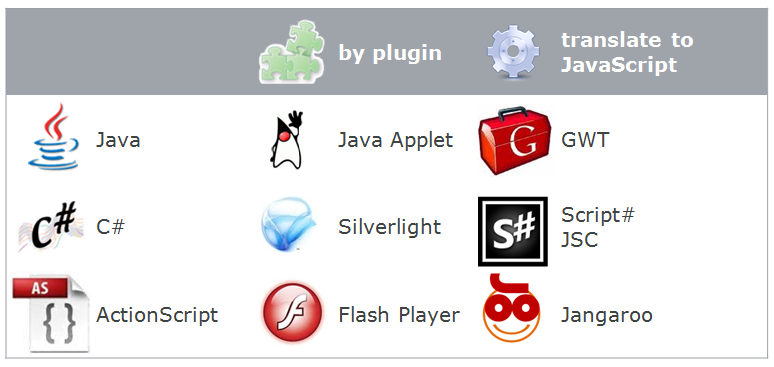
\includegraphics[width=80mm,height=40mm]{TechnologyMatrix.png}
\vspace{20pt}

The fact that ActionScript 3 is actually a superset of JavaScript is a big advantage compared to other tools which target a different high level language like Java or C\#. Here, the high level language is semantically so far away from JavaScript that either a browser plug-in is needed (providing a dedicated virtual machine for execution), or JavaScript code is generated so cryptic that it can only be debugged effectively when using proprietary tools. Also, the semantic gap between the high level language and JavaScript is so wide that only a quite restricted subset of the high level language can be supported if translating to JavaScript. Last but not least, the more the source language differs from JavaScript, the more likely it is that compilation results in inefficient, bloated code that does not use the strengths of JavaScript.

Representatives of another approach consist of a virtual machines implemented in JavaScript, interpreting the same byte code as their plug-in relatives. As of today, Google's Swiffy\citep{swiffy} and Gordon\citep{gordon} simulate only a very old and limited version of the Flash player virtual machine (version �8). 

Mascara\citep{mascara} and haXe\citep{haxe}, like Jangaroo, start with source languages that provide extensions to JavaScript similar to ActionScript, and compile these to Java\-Script. The disadvantage is that both languages,  ECMAScript 4 (Mascara) and haXe's proprietary language, are not widely supported by development tools. ActionScript 3, on the other hand, has broad tool support, which even improved since Adobe introduced Flex\citep{flex}. 

\section{Outlook}

Although ECMAScript 5 did not introduce classes or packages, and it is unlikely to do so in successor versions within the next few years, the enhancements in recent versions of JavaScript even before ECMAScript 5 help simulating ActionScript 3 features. The latest versions of all major browsers now fully support control over properties: accessors (getter/setter functions), custom non-enumerable properties, and read-only properties. ECMAScript 5's \emph{frozen objects} help to simulate ActionScript 3 classes more accurately. Thus, Jangaroo will not become dispensable, but on the contrary, it will be possible to approach full support for ActionScript 3 in modern browsers. 

So far, Jangaroo is proposed mainly as a better way to implement frameworks and large scale software that targets JavaScript environments. But several experimental applications\citep{jangaroo-applications} show that original ActionScript 3 code can � with very few to no changes � be compiled and run in the browser, too. Besides supporting the language, Jangaroo also supports a subset of the Flash libraries with the JooFlash project\citep{jlwiki}. The closer Jangaroo gets to full ActionScript 3 support, the more ActionScript frameworks and applications can easily be ported to run directly in the browser and seamlessly interact with JavaScript code.

Another recent trend is to run JavaScript outside of the browser, for example in Web servers (Node.js\citep{nodejs}, a pioneer was Helma\citep{helma}). The most obvious advantage is that client and server use the same language and can share or even exchange code. Obviously, Jangaroo can be applied in this domain as well, so that both client and server would be implemented in ActionScript. Considering the large and growing number of APIs offered in a server context, working with static typing can be especially helpful here.

\appendix

\acks

We thank our colleagues Dennis Homann and Olaf Kummer for helpful comments and suggestions on earlier versions of this paper.

% alternatives: abbrvnat unsrtnat plainnat
\bibliographystyle{unsrtnat}
\softraggedright
\bibliography{jangaroo}

\end{document}
